\renewcommand{\baselinestretch}{1.5}
\fontsize{12pt}{13pt}\selectfont

\chapter{基于ROS的无人机飞控}\label{introduction}

本章首先研究了ROS系统的基础知识,包括其关键的通信机制和仿真环境;其次对飞控软件PX4 software进行了研究,在整体框架的基础上着重分析了影响飞行的FailSafe机制、EKF2决定的飞行模式和MAVROS控制下的Offboard程序。

\section{ROS}
本节主要对ROS平台进行介绍,包括ROS核心的消息机制和研究中要用到的gazebo仿真平台。

21世纪开始,随着人工智能研究的发展,催生出了一批智能机器人的研究项目;ROS诞生于2007年斯坦福大学AI实验室Morgan Quigley的STAIR(Standford Artificial Intelligence Robot)项目,其期望构建一个基于移动机器人+机械臂的原型;该项目于2008年受到Willow Garage公司关注,其决定用商业化手段来推进机器人的发展,使机器人平台能够更快地走进人们的日常生活;Willow Garage接手该项目后两年,2010年第一代ROS即ROS1.0发布;2013年,OSRF(Open Source Robotics Foundation)接管了ROS的维护工作和版本的升级工作,随后至2018年间,ROS的Indigo、Kinetic和Melodic版本相继发布。

\subsection{ROS整体框架}

ROS即Robotics Operating System,是一个针对机器人的开源、元级操作系统,在某些方面,ROS更像是一种机器人框架(robot framework);它提供类似于操作系统的服务,如图\ref{fig-ros}所示,包含底层的驱动程序管理、底层的硬件描述,随后上升到软件程序之间的消息传递、功能包的管理和发布、也提供用于获得、编译、编写和多设备跨计算机运行代码所需的库等。换言之,ROS是由一套通信机制,开发工具,一系列应用功能和一个庞大的生态系统组成的集合,其目标为提高机器人研发中的软件复用率,不断完善他人的工作,进行更好的开发。

\begin{figure}[!ht]
	\centering
	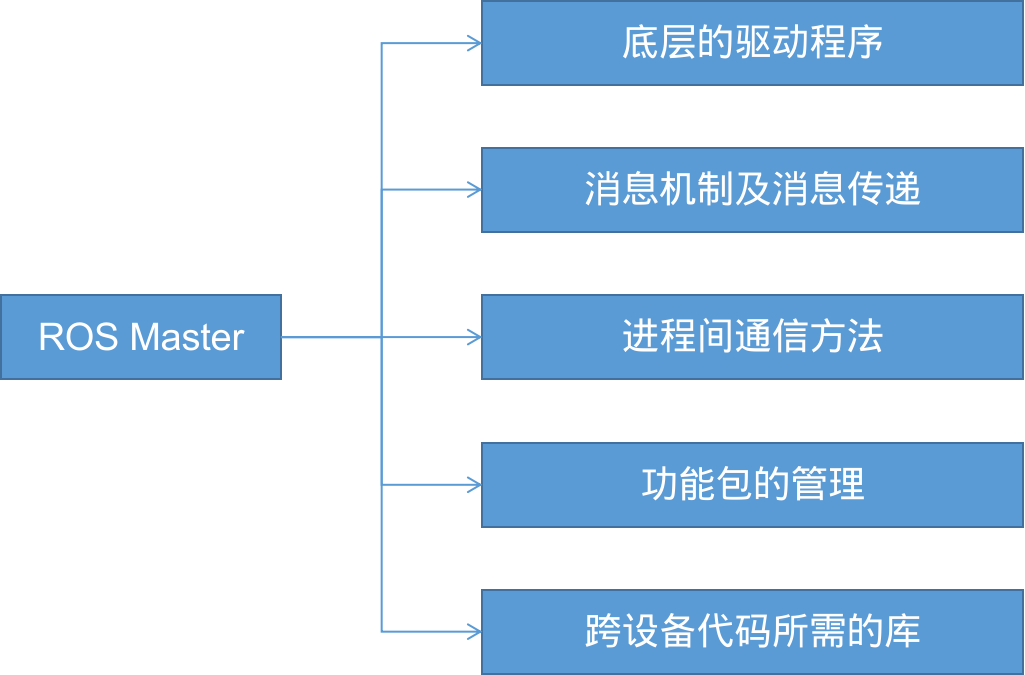
\includegraphics[width=0.6\textwidth]{ros.png}
	\caption{ROS整体框架} 
	\label{fig-ros}
\end{figure}

ROS系统可以分为三个层面,计算图、文件系统和社区:
\begin{enumerate}
	\item 首先是计算图,这一概念主要应用于描述其消息机制;概括地说,是从节点到节点的消息传递,涉及其中通信的方式,数据的类型等内容。
	\item 其次是文件系统;ROS创建了以功能包为核心,配置以CMakeList文件,通过ROS的编译方法快捷完成编译,连接到可执行文件;除此之外,还可以包含python脚本、launch文件和用户自定义的消息和话题类型文件。
	\item 最后是社区级;ROS不仅是一个强大的开源操作系统,也是一个包含了衍生内容的庞大社区;首先,ROS通过不断更新的发行版构成自身的主体;同时,配备有各式软件库,满足用户不同的任务需求;关键是有自己的ROS wiki\footnote[1]{http://wiki.ros.org/}和ROS论坛,十分方便用户查阅学习以及提问;总言之,拥有良好的开发生态。
\end{enumerate}


\subsection{ROS的消息机制} \label{2.1.1}

% ROS松耦合分布式通信+引出节点
ROS提供了一套松耦合分布式通信机制,这种分布式处理框架(又名Nodes),是以多个节点及节点之间的通信组成的。其中,节点(Node)和节点管理器(ROS Master)是ROS的核心概念,若干个节点在节点管理器下构建起来,共同实现特定的功能。

% 介绍节点的作用
每一个节点是一个独立的执行单元,由可执行文件构成,在程序中需要声明节点的名称;节点的名称必须唯一,否则ROS会舍弃掉时间节点靠前的节点;节点执行具体的任务进程,比如单目的ORB-SLAM2中,其节点为Mono,SLAM的任务仅靠一个节点完成。

% 介绍节点管理器
节点管理器是节点的控制中心,其作用是辅助节点的查找,帮助节点之间建立通信连接;还能提供节点的命名和注册等服务,以及提供了能够存储全局变量的配置的参数服务器。

\begin{figure}[!ht]
\centering
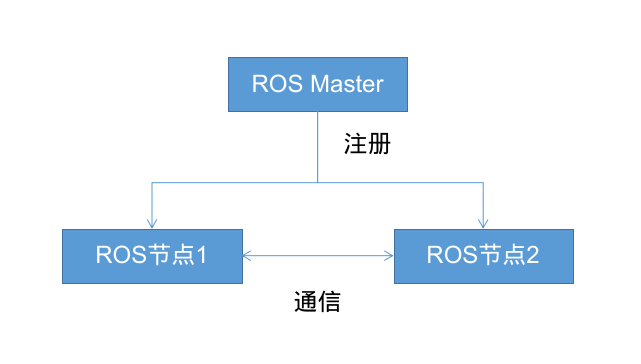
\includegraphics[width=0.6\textwidth]{ros_node.png}
\caption{ROS中的节点及通信} 
\label{fig2}
\end{figure}

% 介绍节点的通信
如图\ref{fig2}所示,节点在经过节点管理器注册后,可以建立节点之间的通信;常用的节点之间通信方式有两种,为话题(Topic)通信和服务(Service)通信:
\begin{enumerate}
	\item 话题通信是异步通信机制,数据为单向传输;数据的流向为发布者(Publisher)到订阅者(Subscriber);完成话题通信需要定义一个话题(Topic)及其消息(Message)的内容,之后通过发布者(Publisher)发布该话题,并且订阅者(Subscriber)订阅该话题的操作,完成数据的传输,消息的数据结构由.msg文件定义;话题通信可以完成多对多的信息传递。
	\item 
	服务的通信机制则为同步,数据为双向传输;数据的流向为客户端(Client)与服务器(Server)之间的交互;完成服务的通信需要客户端向服务器发送请求,服务器完成任务处理后,向客户端返回应答数据,表示请求和应答的数据结构定义在.srv文件中;服务通信一般用于逻辑判断,比如询问一项任务是否执行完毕,是一对多的节点处理关系。
\end{enumerate}

% 介绍Topic的编程
发布和订阅话题的方法,发布者和订阅者类似,以发布者为例:先实例化一个发布者对象,定义发布的话题名称、数据类型和队列长度,最后对消息进行定义并发送,简单的逻辑代码如下:

\begin{minted}[fontsize=\small]{cpp}
ros::NodeHandle n;  // define ros node handle
// define a publisher
ros::Publisher pub = n.advertise<'message type'>
("topic name", `queue length`);
// publish message
pub.publish(message);
\end{minted}

需要注意的是,订阅者则需要声明并定义一个回调函数,在实例化Subscriber的对象后,通过ROS的spin()函数,循环等待回调函数获得话题消息。

% 介绍Service的编程
客户端-服务器模型下的服务通信,则比话题的发布和订阅复杂;客户端的编程实现中,需要设置阻塞函数,其作用是直到发现对应的服务时才向下进行,否则程序被截止在该位置;如果对应的服务被发现,阻塞函数通过,之后创建客户端并且进行数据的设置,完成服务调用的请求,其代码实现如下:

\begin{minted}[fontsize=\small]{cpp}
// wait for right service
ros::service::waitForService("service name");
// create a client, connecting to service
ros::ServiceClient client = n.serviceClient
<'data type'>("service name");
// call service
client.call(srv);
\end{minted}

服务器的实现与订阅者类似,需要一个回调函数,如果收到了客户端发来的请求,则会触发回调函数,程序向下进行,否则将循环等待回调函数收到客户端发来的请求。

% 介绍参数服务器
除此之外,ROS中还有参数(Parameter)或参数服务器的概念,其作用类似全局共享字典,节点可以进行访问,适合存储一些和系统配置相关的静态非二进制的参数,以供节点读取。


\subsection{Gazebo仿真} \label{2.1.2}
% 简单介绍gazebo及其功能
gazebo是ROS自带的仿真软件,其功能有构建具有运动属性的机器人仿真模型,提供了一些针对CAD和soildworks等2D、3D设计软件的接口;gazebo还具有构建现实世界的各种场景的仿真模型的功能,能够在gazebo环境中建立一个与现实十分相似的场景用于算法验证;在传感器的仿真上,gazebo拥有一个强大的传感器模型库,比如单目相机、双目相机、深度相机等,还可以根据需求自行配置传感器的类型,实现多传感器融合;除此之外,gazebo还引入了现实世界的物理性质,如重力的影响,使仿真环境更加贴近现实。

gazebo的仿真环境中,其文件大致可以分为三种类型:model,world,launch文件;同时,这三种文件也代表了不同的分级;

\begin{figure}[!ht]
	\centering
	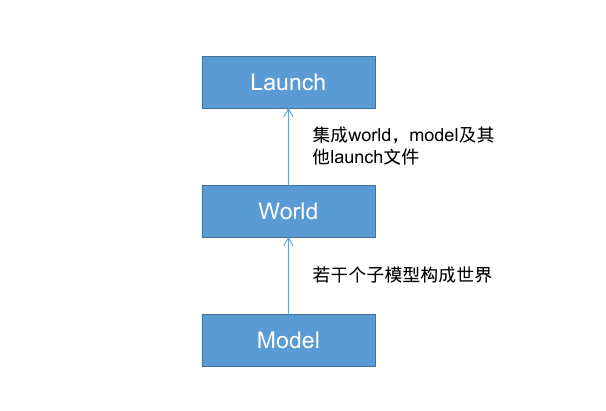
\includegraphics[width=0.6\textwidth]{gazebo.png}
	\caption{model,world,launch层级关系} 
	\label{fig3}
\end{figure}

如图\ref{fig3}所示:
\begin{enumerate}
	\item model(模型)是gazebo环境中的元级元素,也就是最底层文件,比如环境中的树木、双目相机、无人机、墙壁、桌子等都是model级别的物体。model由sdf文件和config文件构成;sdf文件用HTML或XML标签语言描述了该模型的主要内容,包括模型的构建方法、模型中对其他模型的调用以及连接方式、模型的位姿等参数配置;而config文件中记录了模型的作者及联系方式、模型的版本、模型的命名和描述等信息。由于模型具有可拼接的属性,因此一个模型可以由若干个模型组成。
	\item
	world(世界)文件将模型集成起来,包含模型和物理性质的设置,是gazebo环境中的中层文件。该层与model层相同,都无法完成代码对模型的直接控制。
	\item 
	launch文件是集成了model,world以及其他launch文件的gazebo中最顶层的文件;launch文件不同于model和world文件,其可以通过代码完成对模型的直接控制;launch文件在ROS中拥有定义,其以XML标签语言书写,可以在launch文件中完成嵌套其他launch文件、命名重映射、设置参数、启动ROS节点等任务;在ROS中有与launch文件对应的指令roslaunch,用于启动该launch文件。
\end{enumerate}

% 是否还需要一些别的内容

\subsection{工作空间与功能包的使用}

ROS的工作空间是进行开发的基础,后续的所有任务基本都基于工作空间完成。早期的ROS支持rosbuild和catkin两种架构的编译模式,但现今越来越支持catkin的编译,rosbuild逐渐被淘汰,但仍然保留;本文也全部使用的是catkin架构。

工作空间的创建可以使用catkin\_make方法\footnote[1]{http://wiki.ros.org/catkin/Tutorials},但是需要注意python版本,如果要使用python3,则有特殊的编译方法。也可以在src目录下使用catkin\_init\_workspace命令,获得初始化的工作空间。

工作空间一般分为四个部分,如图\ref{fig-catkin}所示,分为src、devel、build、install。在这之中,最常接触到的是src,也就是存放功能包的目录;其次是build,默认功能包编译后会放在这个目录中;devel作为编译后的启动设置文件,一般只在设置环境变量时使用,而install一般是具有发行版后才会使用。除此之外,还可以自己设置一个scripts脚本文件夹,用于快速启动各类程序。
~\\
\begin{figure}[!ht]
	\centering
	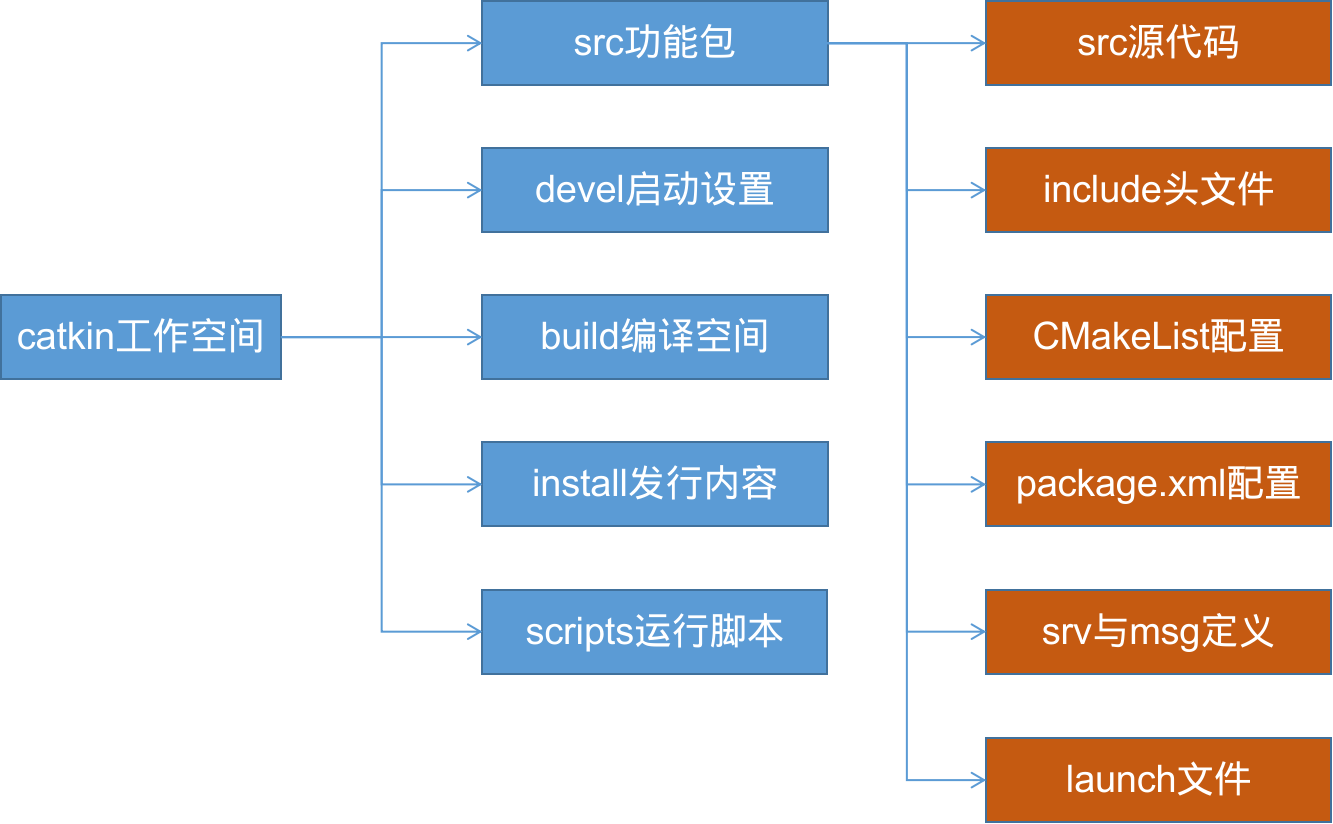
\includegraphics[width=0.7\textwidth]{catkin.png}
	\caption{ROS工作空间结构} 
	\label{fig-catkin}
\end{figure}

ROS开发的关键在于设计功能包,这也符合其设计理念,即提升软件的复用率,避免重复开发。生成功能包的方法如下:

\begin{minted}[fontsize=\small]{shell}
$ catkin_create_pkg <package name> [depend1] [depend2]
\end{minted}

其中,package name为用户定义的功能包名称,depend为该功能包需要的依赖项,一般有roscpp、rospy等;用户后续也可以根据自身需求,在CMakeList中添加相应的依赖。
功能包除了src源代码和其头文件外,还包含package.xml文件,也负责管理依赖,语法和CMake有所区别;还包括srv和msg文件,这些都是由用户定义的服务或消息类型;最后可能会在launch文件夹中添加一些launch文件的用法,用于整体加载参数、启动各节点等。


\section{PX4 AutoPilot飞控软件}
% 本部分介绍PX4
PX4是一款专业级开源飞控,也可以称之为自动驾驶仪;因其应用的平台不局限于飞行器,在竞速和物流应用的地面车辆和潜水艇等载具上也可以用其进行控制。PX4由来自学术界和业界的顶级开发商开发,并且配套有活跃的全球论坛社区,其software的源码在github上保持着issue和pull request的更新,是应用十分广泛的一款飞控软件。需要注意,PX4 Software和Pixhawk4并不是同一概念,前者为飞控软件,而后者为飞控硬件。PX4软件的内部包含了针对不同机型(包括多旋翼、固定翼和VTOL垂直起降固定翼等)的控制律设计,还包含了强大的飞行模式设计和安全设计。PX4还可以作为核心应用在更广阔的平台,比如使用了QGroundControl地面站、Pixhawk硬件、基于计算机、相机等的使用MAVLink协议的MAVSDK融合等\cite{meier2015px4}。

\subsection{PX4整体框架}

PX4的架构可以分为两个部分:一是飞行控制栈,主要包含飞行控制系统和状态估计算法\footnote{https://docs.px4.io/master/en/concept/architecture.html};二是中间控制通信层。主要涵盖嵌入式设备的驱动程序,与外部的通信以及PX4的uORB消息总线。系统支持多种机型和设备,但使用的是一套代码库,并且采用了“响应式”的设计理念,也就意味着其做到了所有功能都可以向下分割成若干可以复用和按需求替换的组件、并且通过异步的方式进行通信,这样的设计也使得系统在不同工作负载下可以有不同的应对方法。以下分别研究飞行控制栈和中间通信层。
~\\
\begin{figure}[!ht]
	\centering
	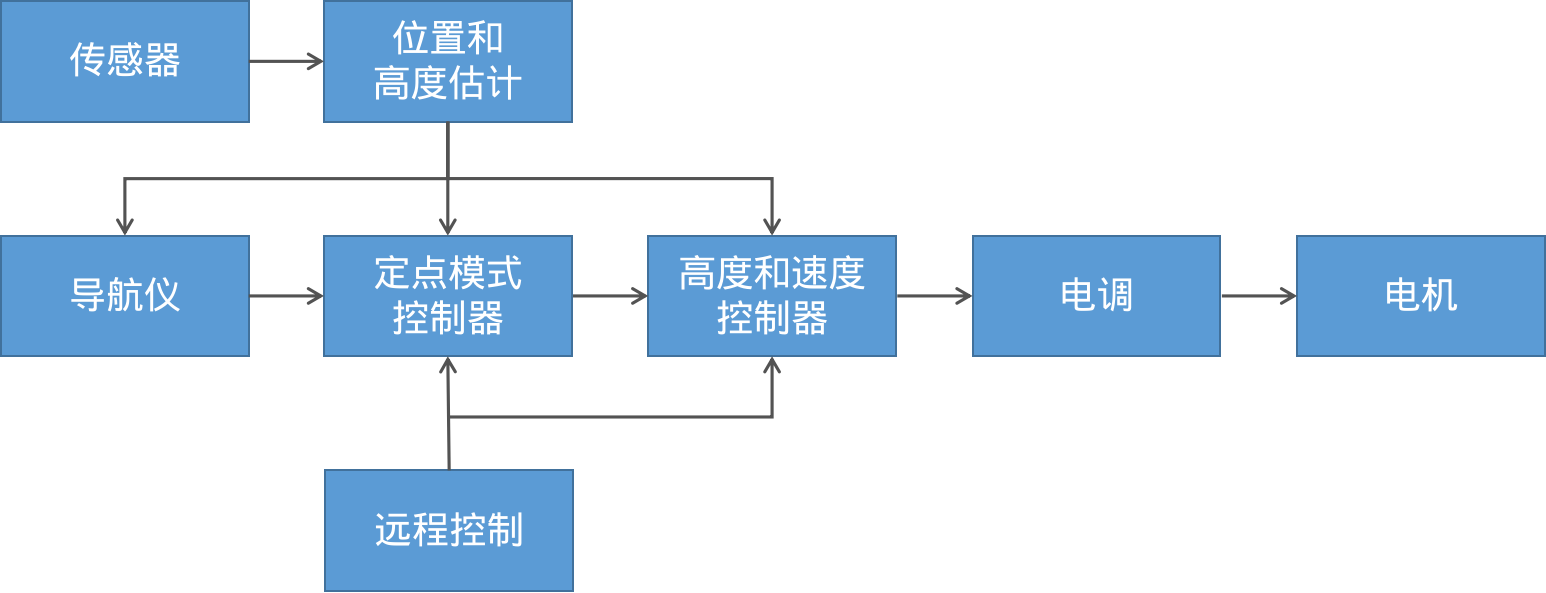
\includegraphics[width=0.9\textwidth]{px4structure.png}
	\caption{飞行控制栈的结构} 
	\label{fig-px4structure}
\end{figure}

飞行控制栈的主要内容如图\ref{fig-px4structure}所示。其中,每个模块意味着不同的功能。箭头表示的是信息流的连接;在信息的传递中,使用uORB总线发布和订阅所有模块之间的相互通信,这样的并行通信可以保证数据抵达后的更新,保证线程进行时的安全。

飞行控制栈是全自主无人机的导航与控制算法的集合。其状态估计首先接收传感器数据,一般有IMU的速度和气压计的高度信息等;之后EKF2根据多个不同传感器的输入,计算出无人机当前的状态,并将计算得到的位姿信息传递给下游的导航控制仪、定点控制器和高度速度控制器。接下来有两种选择,由导航控制仪完成控制或由远端完成控制;导航控制仪意味着完全自主的飞行模式,其将状态估计得到的位姿信息与任务信息比对,并给定点控制器发送下一步指令,定点控制器解算出相应的高度与速度控制信息,传递给电调;电调将上游的指令转换为电机的PWM波指令,这种转换中考虑了系统的动力学模型(传递函数),最终得出确定的控制量,由电机完成更改。

中间控制层包含有存储、外部连接和驱动:
\begin{enumerate}
	\item 存储涵盖有数据库,比如任务信息和地理围栏信息;另一方面存储了参数,这些可以放在ROS的EEPROM虚拟参数缓存中,也可以放在设备的SD卡中;还有一些登录信息。
	\item
	外部连接则主要包括MAVLINK与FastRTPS;前者通过UDP或UART进行连接通信,是本研究中主要使用的方式。
	\item 
	驱动则需要根据无人机搭载的设备而定;一般来说,GPS、相机控制驱动、远程控制和IMU驱动都是包含在内的,还可能有一些机械臂等设备的驱动程序。
\end{enumerate}


\subsection{FailSafe机制} \label{2.2.1}
% 简单介绍FailSafe
FailSafe机制,即安全生效机制,其含义为:当错误发生时,对飞机进行保护或恢复到安全的状态,避免错误可能导致的不良后果。PX4的FailSafe系统是可编辑的,意味着开发者可以根据自身的需求设置对FailSafe的触发,以保证在安全的情况下实验或完成任务。FailSafe系统被触发后,一般有自动着陆、保持位置或返回特定的航路点几种反馈措施。

安全生效机制监控的主要情况有:
\begin{enumerate}
	\item 低电量;该情况在仿真中影响较小,但在真机实验中,低电量可能意味着无法安全返航,因此必须由安全生效机制介入;
	\item 远程控制信号丢失,如遥控器信号丢失;
	\item 位置信息丢失,比如GPS信号弱,对位置的估计不够精确,可能会影响任务的完成情况,因此由安全生效机制介入;
	\item 场外连接丢失;是指进入到Offboard模式后,丢失了与计算机之间的连接,导致计算机无法通过Offboard程序对无人机进行控制;
	\item 数据链丢失;一般是指丢失了与GCS(Ground Control Station,地面站)之间的数传连接;
	\item 超出地理围栏;Geofence即地理围栏,是执行任务前设置的无人机可活动区域,高度一般不设限;
	\item 任务判断;防止在新的起飞位置上执行先前的任务;
\end{enumerate}

% bug实例
PX4版本更新后,如果直接输入commander takeoff指令,可能会遇到无法起飞的情况;同时在PX4终端中,会提示FailSafe activated,即安全生效模式被激活;一般遇到这种情况,需要在PX4终端的字里行间和地面站QGC的信息提示中去分析问题原因。比如在仿真中遇到No RC的情况,RC即Remote Control,对于SITL(软件在环仿真)是没有遥控器的信号输入的,因此需要在QGC中打开virtual joystick (虚拟摇杆),否则FailSafe模式会由于没有RC保持给飞机上锁。

\subsection{EKF与飞行模式} \label{2.2.2}

% 什么是ECL EKF
一般ECL与EKF会同时出现,ECL即Estimation and Control Library,状态估计和控制库;EKF即Extended Kalman Filter,扩展卡尔曼滤波,是一种优化算法。两者的结合是使用扩展卡尔曼滤波方法的状态估计与控制库,其作用是加工传感器的数据,并对IMU(惯性测量单元)加工的速度和位置、四元数表示的旋转矩阵、风速和磁罗盘得到的方向等信息进行加工处理和估计。EKF使用IMU、磁力计、高度计、GPS、测速仪等传感器。

为了将传统的气压计+GPS的高度与位置估计更改为使用视觉信息的高度与位置估计,需要修改EKF传感器的相关参数,这里指用于多旋翼和固定翼的基于扩展卡尔曼滤波的高度和位置估计。

\begin{enumerate}
	\item 
	\textit{EKF2\_AID\_MASK} (Integer bitmask controlling data fusion and aiding methods),该参数决定了GPS数据的融合方法;默认设置的参数为0,其意为使用GPS数据作为定位;如果修改为视觉定位(vision position fusion),需要将该参数改为3。
	\item 
	\textit{EKF2\_HGT\_MODE} (Determines the primary source of height data used by the EKF),该参数决定了EKF首选的高度信息传感器;默认参数设置为0,使用气压器得到高度;如果修改为视觉定位,则需要将该参数改为3。
\end{enumerate}

在启动仿真之前,需要根据信息融合的类型更改以上两个参数,修改参数的方式有以下两种:
\begin{enumerate}
	\item 更改rcS文件中的参数配置;rcS文件属于脚本文件,用于配置系统,PX4需要修改的rcS文件位于\textit{ROMFS/px4fmu\_common/init.d-posix/rcS}中,rcS文件中的参数被修改后,需要删除ROS的eeprom中存储的参数文件(该文件用于快速预加载参数);但该方法存在一些问题,需要在launch中特殊指明PX4使用的rcS文件地址,否则PX4会从默认的build文件夹中选择rcS文件进行参数配置。
	\item 
	更改地面站中的参数配置;使用QGC地面站,直接在参数设置中更改位置和高度估计的传感器,这种方式免去了每次更改参数后需要删除ROS参数缓存文件的麻烦。
\end{enumerate}

飞行模式决定了飞行器对RC远程控制输入的回应,以及在全自主的飞行过程中飞行器如何控制自身的运动;飞行模式为操作者主要提供了不同种类和程度的自动控制协助,飞行欧式的切换可以由遥控器和地面站完成。下面介绍几种主要的飞行模式(对于多旋翼无人机):
\begin{enumerate}
	\item 
	Manual/Stabilized Mode,手动/增稳飞行模式;是最常用的飞行模式,手动模式即操纵手通过手中的遥控器(RC)控制飞机的滚转、俯仰、油门和前后左右的移动;增稳模式也是由操纵手操纵,但引入了内部控制律,使得遥控器输入到飞机运动的表现更加平滑、易控,这是由其内部的控制律决定的;一般情况下为了防止飞机过于剧烈的运动,都采用增稳模式进行飞行。
	\item 
	Position Mode,定点模式;其主要特点是当操纵杆释放或回归中心时,飞机会保持在3D空间中的一个定点位置处,并且自动解算出相应的力去补偿风和其他的干扰力。该模式是对于新手最安全的模式。
	\item
	Altitude Mode,定高模式;其主要特点是当操纵杆释放或回归中心时,飞机会保持固定高度,但不会去平衡风等其他干扰所造成的水平位置的漂移。
	\item 
	Offboard Mode,场外模式;指通过电脑连接或地面站连接,使飞机按照设定的位置、速度或高度等参数飞行,该模式通过MAVLink与场外设备传递信息,是仿真中使用的主要模式。
	\item 
	其他模式,如圆轨迹模式、起飞降落模式、跟随模式、返回模式等。
\end{enumerate}

\subsection{联合MAVROS的Offboard模式} \label{2.2.3}
本小节主要介绍在Offboard模式下,使用ROS节点通过MAVROS向PX4发送信息,使无人机起飞降落、按航路点移动等。

Offboard模式下的无人机正常起飞,需要首先解锁,然后切换飞行模式(默认手动模式)到Offboard模式,但是需要在切换模式前,以不低于2$Hz$的频率发布一些设定点(setpoints),具体实现起飞的步骤如下:

\begin{enumerate}
	\item 
	连接FCU(MAVROS),判断的标准是MAVROS消息类中的state是否表示为连接;如果连接上则可以继续执行,未连接上则通过spin()函数循环等待。
	\item 
	设定setpoints的坐标值,并以不低于2$Hz$的频率发送一些点。
	\item 
	解锁,解锁成功后切换到Ofboard模式并起飞。
\end{enumerate}

其程序的实现如下\footnote[1]{https://gitee.com/hazyparker/my-research/blob/master/1\_basic/src/takeoff\_land.cpp}:

首先是需要的头文件定义,其包括了C++的基本库,MAVROS的消息相关库,和ROS库;

\begin{minted}[fontsize=\small]{cpp}
// realize mode switching and anto takeoff and landing

#include <iostream>
#include <ros/ros.h>
#include <geometry_msgs/PoseStamped.h>
#include <mavros_msgs/SetMode.h>
#include <mavros_msgs/State.h>
#include <mavros_msgs/PositionTarget.h>
\end{minted}

之后需要在main函数之前,声明定义回调函数,其中包括对当前状态和当前位置的回调函数和消息定义:
\begin{minted}[fontsize=\small]{cpp}
// record current state
mavros_msgs::State current_state; /* NOLINT */

// callback function for Subscriber stats_sub
void state_cb(const mavros_msgs::State::ConstPtr& msg){
current_state = *msg;
}

// record current pose
geometry_msgs::PoseStamped current_pose; /* NOLINT */

// callback function for Subscriber for local_pos_sub
void local_cb(const geometry_msgs::PoseStamped::ConstPtr& msg){
current_pose = *msg;
}
\end{minted}

在main函数中,首先要定义ROS节点和句柄,实例化飞行模式和当前位置信息的订阅者和发布者,然后以一定的频率发送一些点,以便切换到Offboard模式:
\begin{minted}[fontsize=\small]{cpp}
// init ros node
ros::init(argc, argv, "offb_node");

// create node handle
ros::NodeHandle nh;

// define subscribers and clients
ros::Subscriber state_sub = nh.subscribe<mavros_msgs::State>
("mavros/state", 10, state_cb);
ros::Subscriber local_pos_sub = nh.subscribe<geometry_msgs::PoseStamped>
("mavros/local_position/pose",10,local_cb);
ros::Publisher local_pos_pub = nh.advertise<geometry_msgs::PoseStamped>
("mavros/setpoint_position/local", 10);
ros::ServiceClient arming_client = nh.serviceClient<mavros_msgs::CommandBool>
("mavros/cmd/arming");
ros::ServiceClient set_mode_client = nh.serviceClient<mavros_msgs::SetMode>
("mavros/set_mode");

//the set-point publishing rate MUST be faster than 2Hz
ros::Rate rate(20.0);

// wait for FCU connection
while(ros::ok() && !current_state.connected){
    ros::spinOnce();
    rate.sleep();
    ROS_INFO("wait for fcu connecting...");
}
ROS_INFO("fcu connected successfully");

// set pose
geometry_msgs::PoseStamped pose;
pose.pose.position.x = 0;
pose.pose.position.y = 0;
pose.pose.position.z = 2;

//send a few set-points before starting
for(int i = 100; ros::ok() && i > 0; --i){
    local_pos_pub.publish(pose);
    ros::spinOnce();
    rate.sleep();
}
\end{minted}

最后首先发送指令,使无人机解锁,之后使其切换到Offboard模式,完成起飞并到达目标点的指令:
\begin{minted}[fontsize=\small]{cpp}
int main(int argc, char **argv){
    mavros_msgs::SetMode offb_set_mode;
    offb_set_mode.request.custom_mode = "OFFBOARD";

    mavros_msgs::CommandBool arm_cmd;
    arm_cmd.request.value = true;

    ros::Time last_request = ros::Time::now();
    ROS_INFO("Off boarding");
    
    while(ros::ok()){
        if( current_state.mode != "OFFBOARD" &&
        (ros::Time::now() - last_request > ros::Duration(5.0))){
            if( set_mode_client.call(offb_set_mode) &&
            offb_set_mode.response.mode_sent){
                ROS_INFO("Off-board mode enabling...");
            }
        last_request = ros::Time::now();

        } else {
            if( !current_state.armed &&
            (ros::Time::now() - last_request > ros::Duration(5.0))){
                if (current_state.mode != "OFFBOARD") ROS_INFO("Off board mode down");
                if( arming_client.call(arm_cmd) && arm_cmd.response.success){
                    ROS_INFO("Vehicle armed");
                }
            last_request = ros::Time::now();
            }
        }

        local_pos_pub.publish(pose);

        // wait until reach set point
        ros::spinOnce();
        // define Point: current position and set point position (expected)
        geometry_msgs::Point curr,aim;
        curr = current_pose.pose.position;
        aim = pose.pose.position;
        double dist = sqrt(pow((curr.x - aim.x), 2) +
pow((curr.y - aim.y), 2) + pow((curr.z - aim.z), 2));
        if(dist < 0.1){
        ROS_INFO("reached the goal...");
        break;}
        rate.sleep();
        }
    }

    return 0;
}
\end{minted}











